\documentclass{beamer}
\usetheme{Boadilla}
\usepackage{graphicx} % Required for inserting images
\usepackage{hyperref}

\title{AP1 et usage d'IA génératives}
\author{Equipe AP1}
\date{September 2026}

\begin{document}

\begin{frame}
    \maketitle
\end{frame}

\begin{frame}{De quoi on parle ?}
    \pause
      \begin{center}
        
\includegraphics[width=0.20\textwidth,height=1.2cm,keepaspectratio]{Images/ChatGPT.png}
        \hfill
        
\includegraphics[width=0.20\textwidth,height=1.2cm,keepaspectratio]{Images/Mistral.png}
        \hfill
        
\includegraphics[width=0.20\textwidth,height=1.2cm,keepaspectratio]{Images/Claude.png}
        \hfill
        
\includegraphics[width=0.20\textwidth,height=1.2cm,keepaspectratio]{Images/Gemini.png}
    \end{center}
       \vfill

    On parle ici des modèles langue/LLM : ChatGPT, Claude, etc. 
7   \pause

    \begin{block}{Comment ça marche ?}
        \begin{itemize}
            \item Option Apprentissage Automatique au second semestre
            \item Des cours plus tard dans vos études
            \item Version vulgarisée \underline{\href{https://elearning.univ-eiffel.fr/mod/page/view.php?id=341001}{sur Elearning}}
        \end{itemize}
    \end{block}


  

\end{frame}

\begin{frame}{Le futur, ou pourquoi utiliser l'IA}

\begin{block}{ Où en sera l'IA dans 5 ans ?}
\pause
Si vous savez, écrivez-moi. 


\pause 
En tout cas, toujours là.
\end{block}

\begin{itemize}
    \item Génération de code simple.
    \item Assistance à la programmation.
    \item Modèles de "réflexion".
    \item Investissement massif des entreprises.
\end{itemize}
\end{frame}

\begin{frame}{Le futur, ou pourquoi ne pas utiliser l'IA ?}

    % Étape 1
    \only<1>{
        \begin{center}
            \textbf{\Large Fiabilité et hallucinations}
            
            \vfill
            
            
\includegraphics[width=\textwidth,height=0.75\textheight,keepaspectratio]{Images/Fiability.png}
        \end{center}
    }

    % Étape 2
    \only<2>{
        \begin{center}
            \textbf{\Large Impact environnemental conséquent}
            
            \vfill
            
            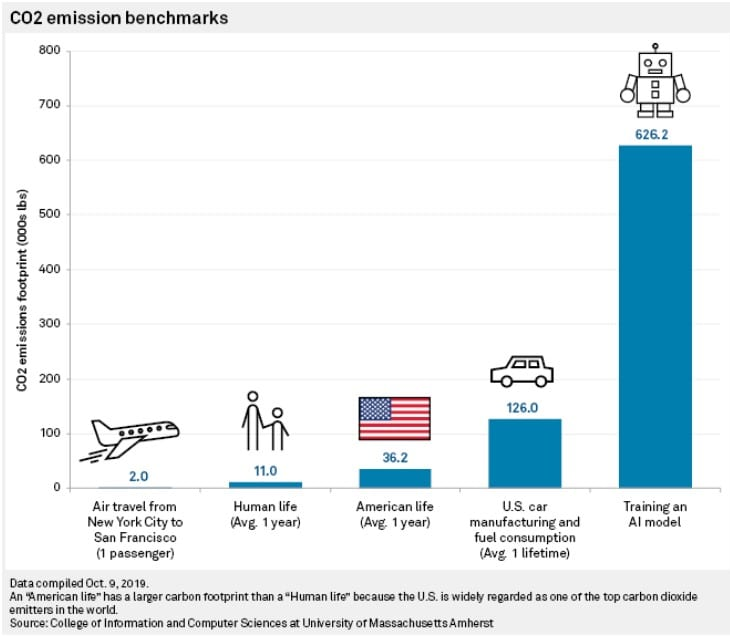
\includegraphics[width=\textwidth,height=0.75\textheight,keepaspectratio]{Images/CarbonImpact.png}
        \end{center}
    }

    % Étape 3
    \only<3>{
        \begin{center}
            \textbf{\Large Monopole de grandes entreprises privées et "gratuité" douteuse}
            
            \vfill
            
            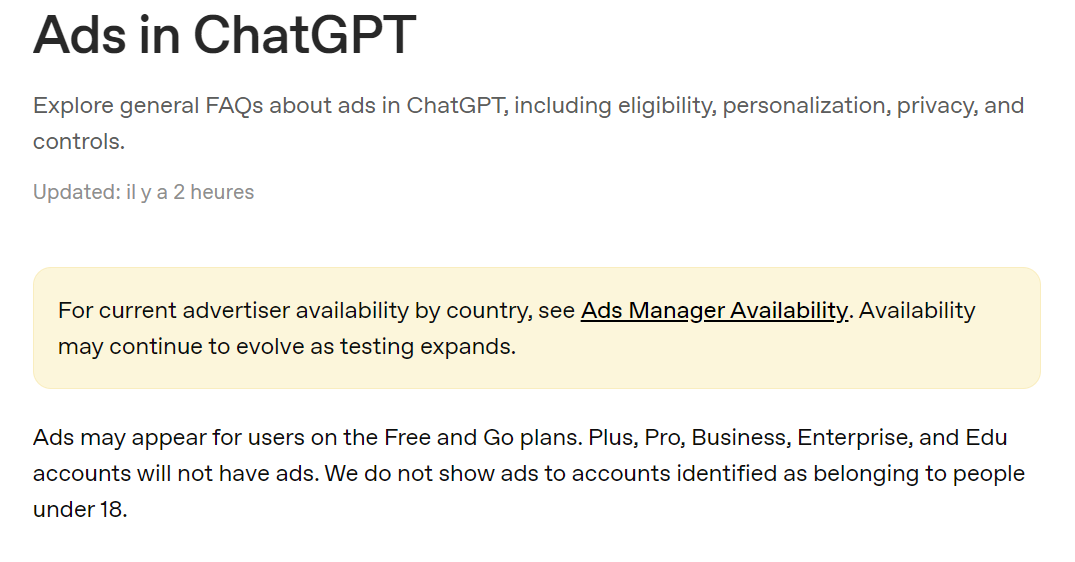
\includegraphics[width=\textwidth,height=0.75\textheight,keepaspectratio]{Images/AdsGPT.png}
        \end{center}
    }

    % Étape 4
    \only<4>{
        \begin{center}
            \textbf{\Large Impact culturel}
            
            \vfill
            
            
\includegraphics[width=\textwidth,height=0.75\textheight,keepaspectratio]{Images/CulturalImpact.png}
        \end{center}
    }

    % Étape 5
    \only<5>{
        \begin{center}
            \textbf{\Large Opacité et partialité des LLMs}
            
            \vfill
            
            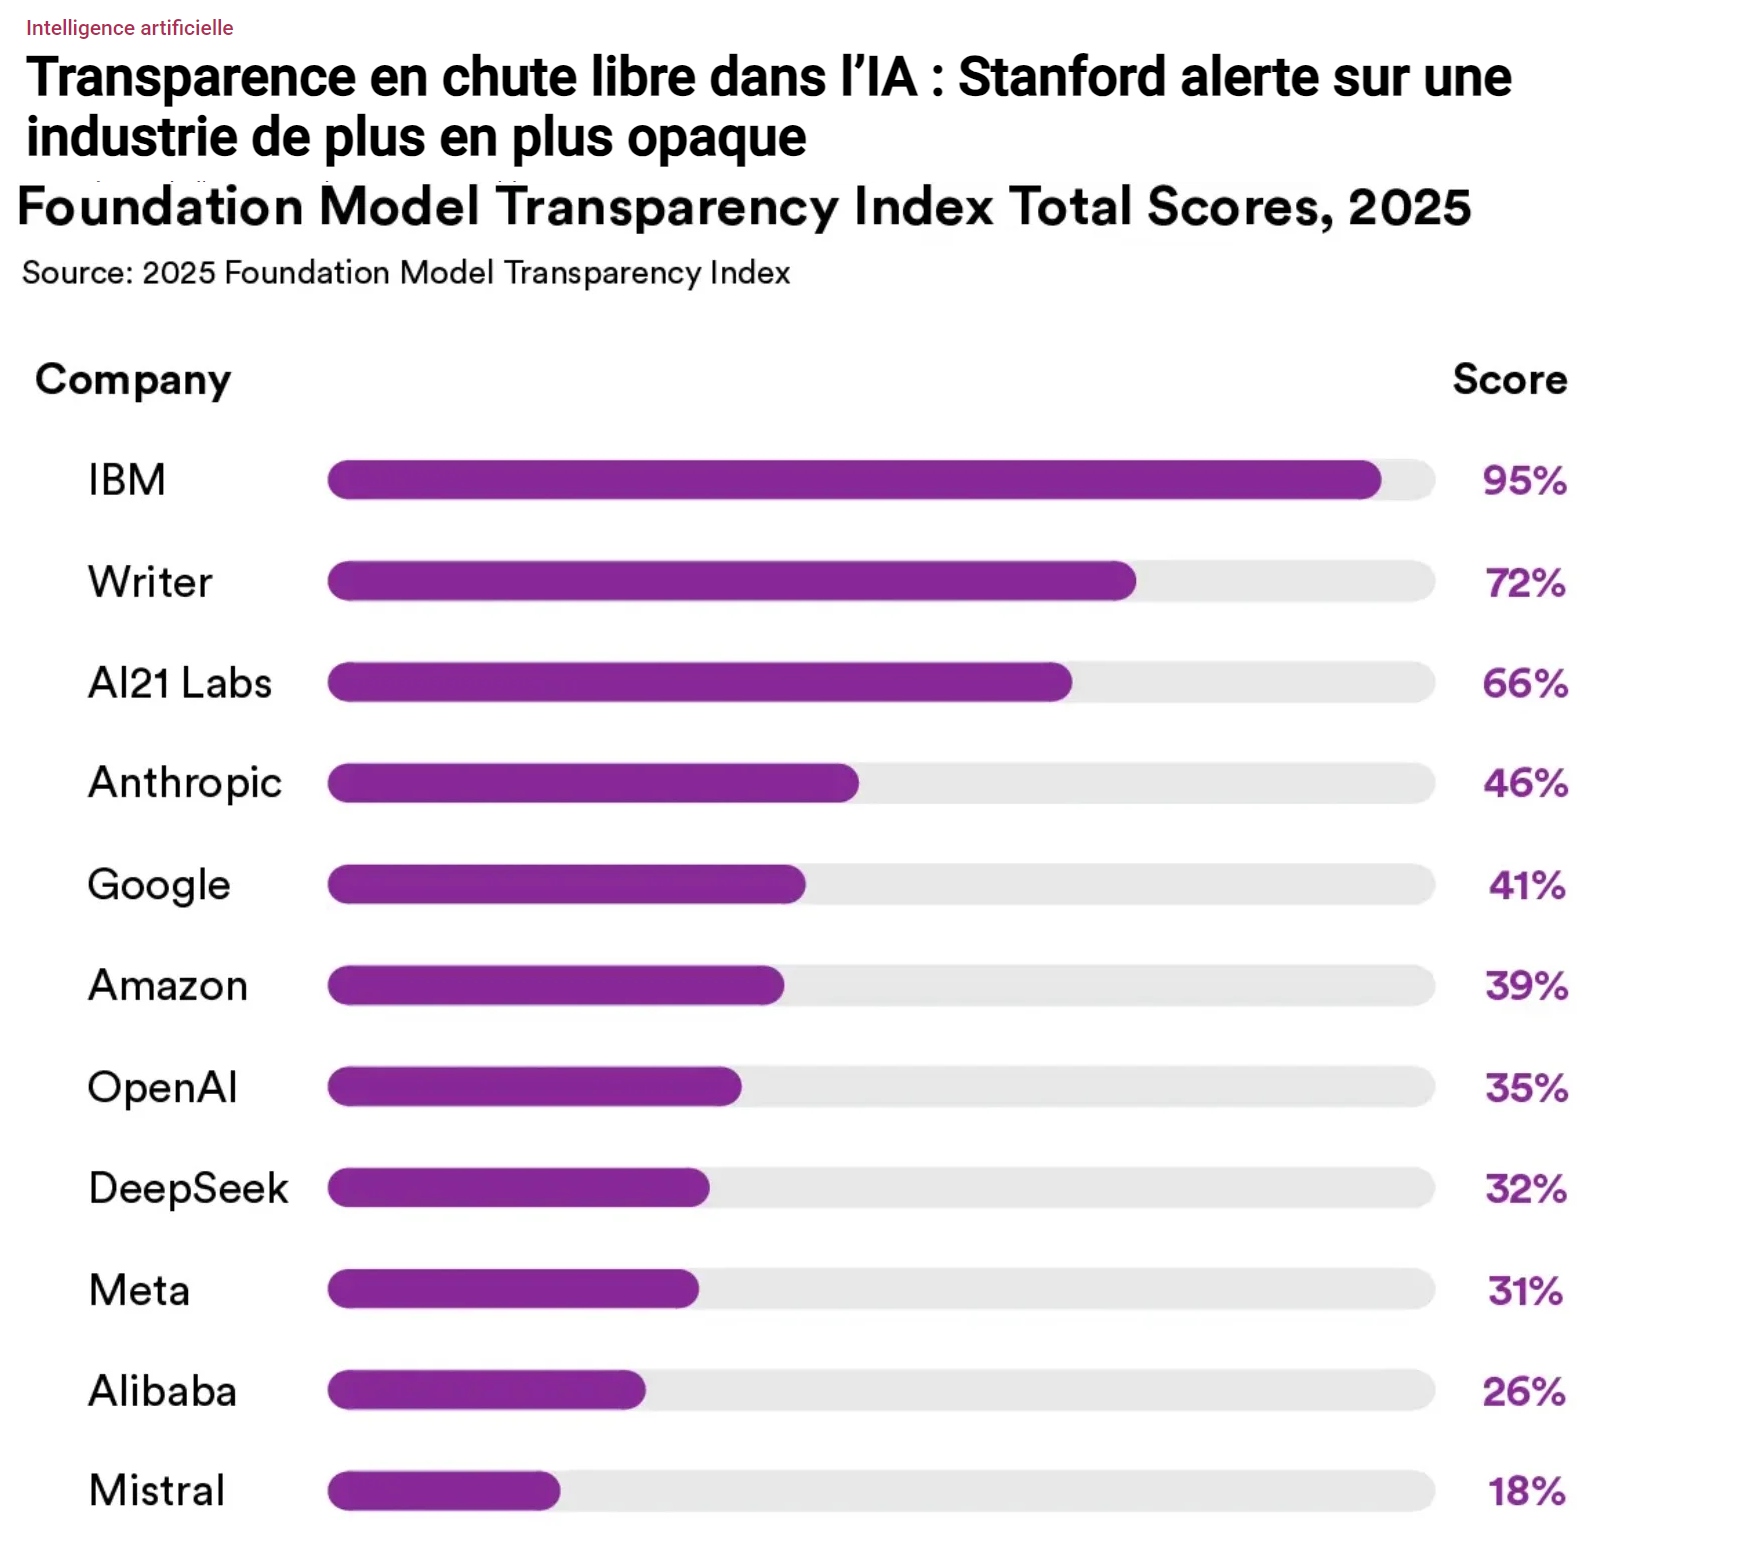
\includegraphics[width=\textwidth,height=0.75\textheight,keepaspectratio]{Images/Opacity.png}
        \end{center}
    }

    \only<6>{

    \begin{center}
            \textbf{\Large Paresse Intellectuelle}
            
            \vfill
            
            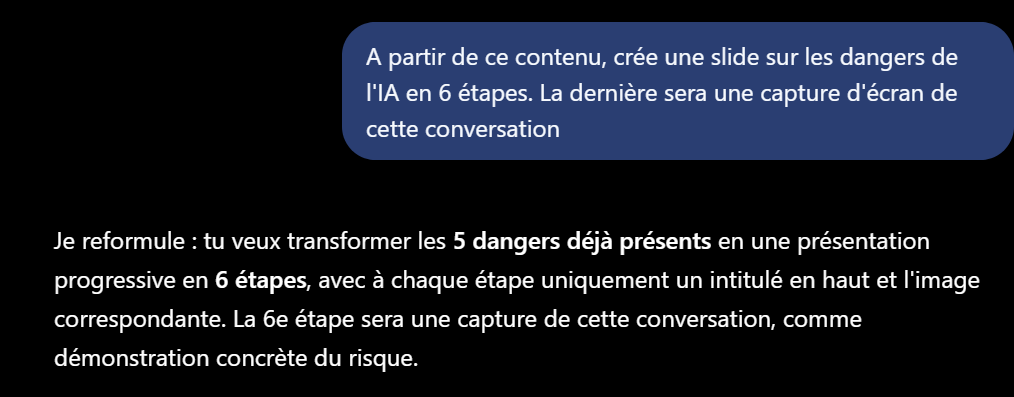
\includegraphics[width=\textwidth,height=0.75\textheight,keepaspectratio]{Images/Paresse.png}
        \end{center}
    }
\end{frame}


\begin{frame}{Là où on en est actuellement : un rapport récent du MIT}

Rapport  accessible \underline{\href{https://aiandeducation.mit.edu/report/}{ici}} (août 2026)
     \begin{itemize}
         \item  Tout ce qui est enseigné au niveau Licence est réalisable par une IA.
         \item Tous les enseignements sont à ré-évaluer.
        \item Les projets maison doivent être beaucoup plus ambitieux.
        \item Important de "bloquer" sur des questions pour progresser.
    \end{itemize}
    
    \pause 
        
    \begin{center}
        \textbf{Est-ce une bonne nouvelle pour vous ? }
    \end{center}
   
\end{frame}

\begin{frame}{Notre posture en AP1}
\begin{center}
    \textbf{L'usage de l'IA n'est ni interdite, ni obligatoire.}
\end{center}
\pause
\begin{itemize}
    \item Son utilisation n'est pas nécessaire pour valider l'année. 
    \item Tous les modèles feront l'affaire. 
    \item Si vous l'utilisez, utilisez la intelligement.
\end{itemize}

\end{frame}

\begin{frame}{Comment utiliser l'IA dans ses études}

  Le principal :
\begin{center}
    \textbf{Les IAs ne doivent pas remplacer votre apprentissage, ni votre envie d'apprendre.}
\end{center}
\pause 
\vfill
Traitez-la comme un prof particulier qui vous aide à comprendre des choses, mais pas qui fait à votre place. 
\end{frame}

\begin{frame}{Do's and Don'ts}

\begin{columns}[T,onlytextwidth]

    % Do's
    \begin{column}{0.48\textwidth}
        \begin{block}{Do's}
            \begin{itemize}
                \item[$\checkmark$] Vous expliquer un concept informatique
                \item[$\checkmark$] Demander des points de syntaxe Python
                \item[$\checkmark$] Donner des indices pour débugguer votre code
                \item[$\checkmark$] Relire et vous aider à structure votre rapport de projet
            \end{itemize}
        \end{block}
    \end{column}

    \hfill

    % Don'ts
    \begin{column}{0.48\textwidth}
        \begin{block}{Don'ts}
            \begin{itemize}
                \item[$\times$] Faire vos exos de TDs pour vous
                \item[$\times$] Ecrire tout votre code à votre place
                \item[$\times$]Tout corriger sans expliquer pourquoi
                \item[$\times$] Générer un rapport de projet de 20 pages. 
            \end{itemize}
        \end{block}
    \end{column}

\end{columns}
\pause
\begin{center}
    En informatique, on apprend en pratiquant. Si vous ne le faites pas, vous compromettez votre succès.
\end{center}
\end{frame}

\begin{frame}{Ce que ça veut dire pour l'évaluation}

    \begin{center}
        \textbf{Vous êtes responsables de ce que vous rendez. Toute ligne écrite doit être comprise.}
    \end{center}


    \begin{center}
        \item Si vous ne savez pas expliquer votre code $\to$ 0.
        \item Si vous ne savez pas ce qui est dans votre rapport de projet $\to$ 0.
        \item Evidemment, usage d'IA à l'examen $\to$ 0 + PV de triche + Interdit d'examen.
    \end{center}
\end{frame}

\begin{frame}{Pourquoi apprendre des choses que l'IA fait mieux que nous ?}

\begin{itemize}
    \item On va aller plus loin, mais vous avez besoin de maîtriser les bases pour aller plus loin.
    \pause\item Si vous n'êtes pas meilleur que n'importe qui avec un LLM, vous n'êtes pas employable.
    \pause\item On ne vous apprend pas que la programmation, mais aussi le raisonnement informatique.
    \pause\item Pour le plaisir d'apprendre et de savoir faire les choses soi-même.
    \pause\item Pour savoir créer les technologies de demain.
\end{itemize}
    
\end{frame}

\end{document}
